%%% CLOUD BUILDER
\subsection{Cloud Foundation Builder VM Support}
\label{subsec:cloudBuilder}


\subsection{Red, almacenamiento y servicios necesarios para el despliegue}

\subsubsection{Servicios internos}
\label{subsubsec:servInterno}
Durante el despliegue Cloud Foundation, hay servicios y puertos deben estar habilitados en cada nodo ESXi para Cloud Foundation Builder (Fig. \ref{fig:puertosCB}) y SDDC Manager (Fig. \ref{fig:puertosSDDC}) puedan acceder a todos los componentes.

%%%%%%%%%%%%%%%%%%%%%%%%%%%%%%%%%%%%%%%%%%%%%%%
\iffalse
\begin{figure}[h!]
  \centering
  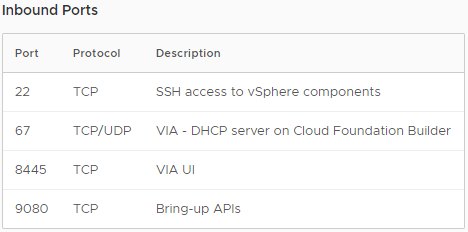
\includegraphics[width=0.7\textwidth]{imaxes/conceptosPrevios/puertosentradaCB.png}
  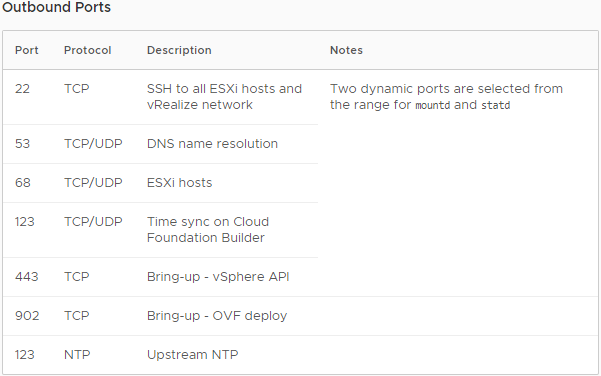
\includegraphics[width=0.7\textwidth]{imaxes/conceptosPrevios/puertossalidaCB.png}
  \caption{Servicios y puertos de entrada y salida habilitados para Cloud Foundation Builder.}
  \label{fig:puertosCB}
\end{figure}

\begin{figure}[h!]
  \centering
  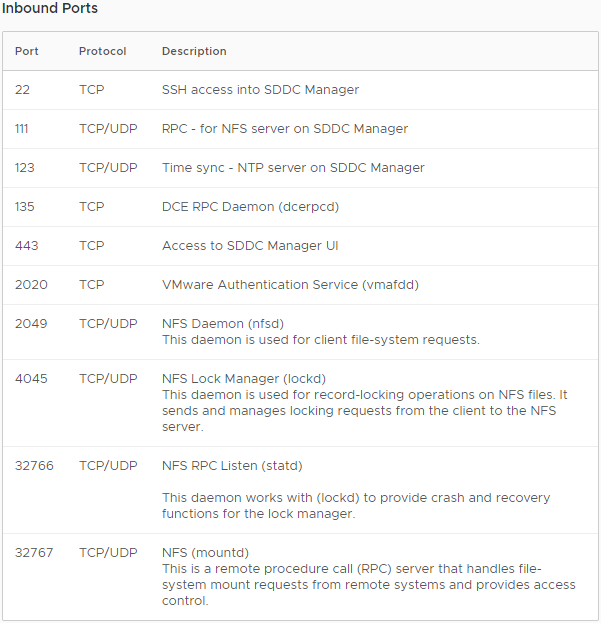
\includegraphics[width=0.7\textwidth]{imaxes/conceptosPrevios/puertosentradaSDDC.png}
  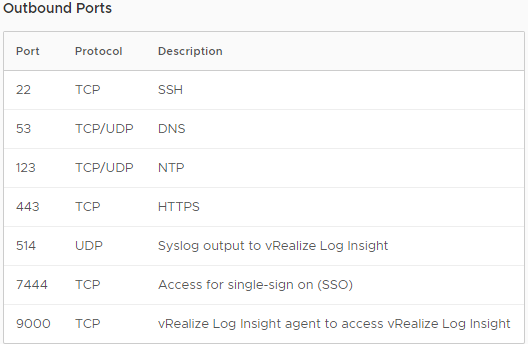
\includegraphics[width=0.7\textwidth]{imaxes/conceptosPrevios/puertossalidaSDDC.png}
  \caption{Servicios y puertos de entrada y salida habilitados para SDDC Manager.}
  \label{fig:puertosSDDC}
\end{figure}
\fi
%%%%%%%%%%%%%%%%%%%%%%%%%%%%%%%%%%%%%%%%%%%%%%%%%%%

\begin{figure}[h!]
  \centering
  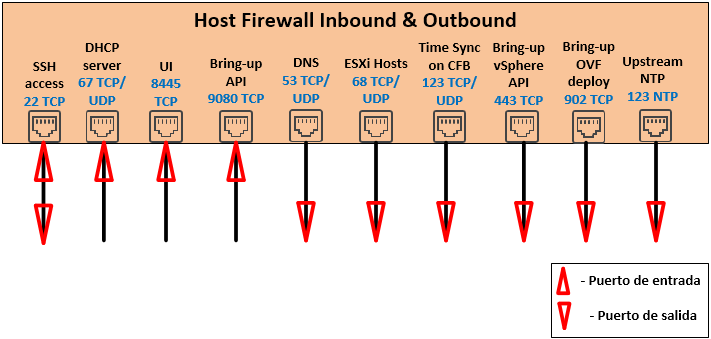
\includegraphics[width=1\textwidth]{imaxes/conceptosPrevios/firewall_CloudBuilder.png}
  \caption{Servicios y puertos de entrada y salida habilitados para Cloud Foundation Builder.}
  \label{fig:puertosCB}
\end{figure}
\begin{figure}[h!]
  \centering
  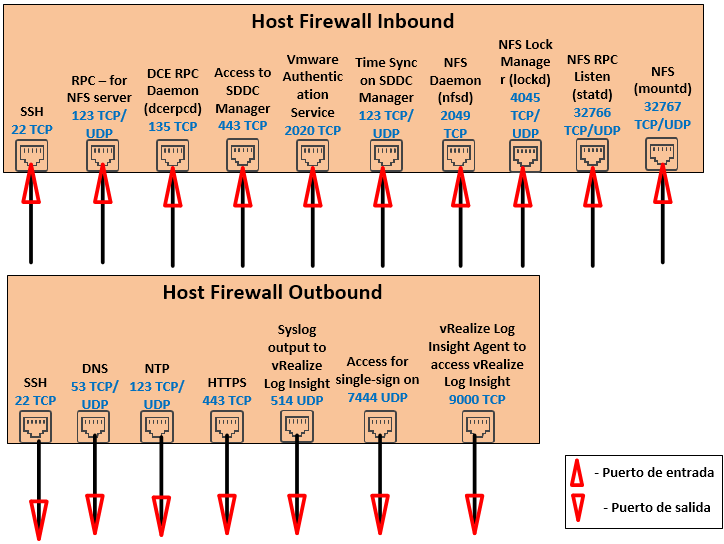
\includegraphics[width=1\textwidth]{imaxes/conceptosPrevios/firewall_SDDC.png}
  \caption{Servicios y puertos de entrada y salida habilitados para SDDC Manager.}
  \label{fig:puertosSDDC}
\end{figure}

\FloatBarrier

\subsubsection{Servicios externos}
\label{subsubsec:servExterno}


Se puede encontrar más información sobre otros servicios opcionales en el siguiente \href{https://docs.vmware.com/en/VMware-Cloud-Foundation/3.9/com.vmware.vcf.planprep.doc_39/GUID-F022BD3C-F11C-4EE6-83EA-ABE016E7A9B9.htm}{enlace}.
\FloatBarrier

%%%%% RED 
\subsubsection{Red física}
\label{subsubsec:redFisica}
La red física debe admitir las siguientes características:
\begin{itemize}
    \item \textbf{VLAN}: etiquetado de redes VLAN (802.1Q)
    \item \textbf{Jumbo Frames}: MTU mínimo igual a 1600, aunque se recomienda que sea igual a 9000.
\end{itemize}

\subsubsection{Red lógica}
\label{subsubsec:redLogicaCF}
\iffalse
Antes del despliegue es necesario especificar varias redes que más tarde Cloud Foundation usará para automatizar la configuración de puertos \ref{Word:vmkernel} cuando se añade un nuevo host al entorno o se crea un VI Domain. Estas redes son  una dedicada al servicio \underline{vSAN}, otra dedicada a \underline{vMotion}, ota de dedicada a la gestión de los componentes y otra dedicada al tráfico de las máquinas virtuales. Los datos a especificar son la etiqueta VLAN, MTU, IP de la red, máscara, gateway y el rango de direcciones IP. Una vez creadas solo se puede modificar el rango de direcciones IP.\\
Es importante utilizar VLANs e IPs ya que es en lo que se basa Cloud Foundation para aislar cada tipo de tráfico de la infraestructura. La cantidad de subredes necesarias depende del número de Workload Domains que se creen, número de clusters y otros componentes opcionales.
\fi

Antes de iniciar el despliegue de VMware Cloud Foundation, el entorno sobre el que se instalará la plataforma debe tener configurado un vSphere Distributed Switch, una llamada \textit{Management Network} que se dedicará a la transmisión del tráfico generado entre los distintos componentes del entorno, y otra llamada \textit{VM Network} que se dedicará al tráfico generado por las máquinas virtuales que se desplieguen sobre la plataforma. La red \textit{Management Network} se puede configurar con etiquetado VLAN, en ese caso la red \textit{VM Network} debe tener la misma etiqueta VLAN. Los vSwitches creados deben tener un MTU igual a 1600 como mínimo. Además, es necesario conocer de antemano las direcciones IP que se asginarán a cada componente de la infraestructura durante el despliegue de la plataforma.
